
\section{Stochastic Shape Grammars}

We will represent a placed symbol $X_{p,q}$ as a labeled line segment:
\mar{labeled line segment}

We will represent a placed terminal symbol $\ell_{p,q}$ as a labeled
line segment whose line is darker.
\mar{labeled line segment}

We will represent a placed curvilinear form by chaining together
labeled line segments. Note that a curvilinear form can consist of a
mixture of placed nonterminal symbols (light lines) and placed
terminal symbols (dark lines).
\mar{labeled curvlinear form}

\mar{Describe depicted grammar}

\begin{figure}
\includegraphics[width=4.0in]{images/grammar-state.eps}
\end{figure}

\begin{figure}
\includegraphics[width=4.0in]{images/grammar-rules.eps}
\end{figure}

\section{A parse tree}

\begin{figure}
\includegraphics[width=5in]{images/parsetree.eps}
\end{figure}
